\scanpage{136}
\[
\mathbb R\unsure{\mathcal Hom|\operatorname{Hom}}(M_\bullet,L_\bullet)\simeq M_\bullet^\vee\overset{\mathbb L}{\otimes}L_\bullet.
\]
et on voit que $\mathbb R\unsure{\mathcal Hom|\operatorname{Hom}}(M_\bullet,L_\bullet)$ et $\mathbb R\unsure{\mathcal Hom|\operatorname{Hom}}(L_\bullet,M_\bullet)$
sont ``duals'' l'un de l'autre au sens
du $\vee$, en particulier ils sont
\uline{accouplés} à valeurs dans $A$. En
particulier, de cet accouplement résulte
si
\[
\begin{aligned}
u&\in H^0(\mathbb R\operatorname{Hom}(\unsure{L_\bullet|M_\bullet},\unsure{M_\bullet|L_\bullet}))=\operatorname{Hom}_{D(A)}(\unsure{L_\bullet|M_\bullet},M_\bullet)\\
v&\in H^0(\mathbb R\operatorname{Hom}(M_\bullet,L_\bullet))=\operatorname{Hom}_{D(A)}(M_\bullet,L_\bullet)
\end{aligned}
\]
un accouplement
\[
\langle u,v\rangle=H^0(A)=A
\]
\deleted{\unsure{Que}\illegible{1}}
Le calcul donne l'explicitation
\[
\boxed{\langle u,v\rangle=\langle v,u\rangle=\sum\deleted{\operatorname{Tr}}(-1)^i\operatorname{Tr}(v\circ u)^i=\sum(-1)^i\operatorname{Tr}(u\circ v)^i}
\]
si $L_\bullet,M_\bullet$ sont \deleted{\unsure{libres}}\inserted{projectifs} de type fini en
chaque degré; \inserted{et $u,v$ \unsure{désignant|désignent} ici des hom. de complexes (dans $K(A)$): qui définissent $u,v$.}
En particulier si $L_\bullet=M_\bullet$
on trouve pour $u\in\operatorname{Hom}_{D(A)}(L_\bullet,L_\bullet)$
\[
\boxed{\sum(-1)^i\operatorname{Tr}u^i=\langle u,\operatorname{id}_{L_\bullet}\rangle=\langle\operatorname{id}_{L_\bullet},u\rangle.}
\]
ce qui fournit bien une expression
intrinsèque de ce $\sum(-1)^i\operatorname{Tr}u^i$ en termes dér.
\margin{\unsure{b|6} Tout est contenu dans la notion plus générale qui suit \dots}
\figure{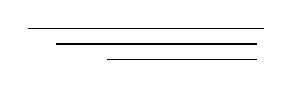
\begin{tikzpicture}\draw (0,0)--(3,0);\draw (.35,-.2)--(2.9,-.2);\draw (1,-.4)--(2.9,-.4);\end{tikzpicture}}
Bien entendu, pour pouvoir appliquer la notion
$\operatorname{Tr}_*u$ dans le contexte de la formule de Lefschetz, il y
faut savoir que $\mathbb R\Gamma_X(A_X)$ est bien \inserted{ps. coh. et} de Tor-dim finie.
\inserted{La pseudo-cohérence est connue, la Tor-dim}
\mspage{135}
